% id: 109-18
% book: 베이직쎈 확률과 통계 · 06 이항분포와 정규분포
% section: 개념 32 정규분포곡선에서의 확률
% passage: 확률변수 $X$가 정규분포 $\mathrm{N}(m{,}\mkern3mu\mathopen{}\sigma^2)$을 따르고\par\smallskip\centerline{$\mathrm{P}(m\le X\le m+\sigma)=a$, $\mathrm{P}(m\le X\le m+2\sigma)=b$}\par\smallskip\noindent 일 때, 다음을 $a$, $b$를 사용하여 나타내시오.
% figure: tikz:fig-109-18
% answer: 
% answer_source: 
% variant_level: 0 (원본 전사)
% 이 파일은 build.mjs 가 items.json 에서 만든다. 고칠 때는 items.json 을 고친다.
\smash{\raisebox{1.5mm}{\dmkichul{베이직쎈 확률과 통계 109쪽 18번}}}
\noindent\begin{minipage}[t]{0.58\linewidth}\vspace{0pt}\raggedright $\mathrm{P}(m-\sigma\le X\le m)$\end{minipage}\hfill\begin{minipage}[t]{0.4\linewidth}\vspace{0pt}\centering \resizebox{\ifdim\width>\linewidth\linewidth\else\width\fi}{!}{% 109-18(인쇄 109쪽) — 힌트의 정규분포곡선: m-σ 부터 m 까지의 넓이(P(m-σ≤X≤m))를 색칠한 그림.
% 스캔 화질이 낮아 TikZ 로 다시 그림. 라벨은 원문에 있는 것만(m-σ, m, x) · 구하는 확률은 그림에 적지 않는다.
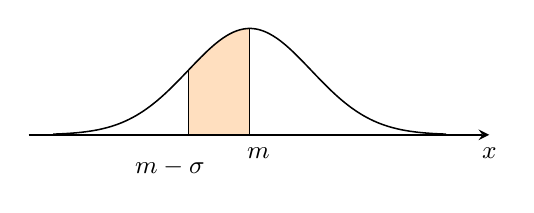
\begin{tikzpicture}[x=0.78cm, y=1.35cm, line width=0.55pt, font=\small]
  \fill[orange!25] plot[domain=-1:0, samples=40, smooth] ({\x},{exp(-\x*\x/2)}) -- (0,0) -- (-1,0) -- cycle;
  \draw[->, >=stealth, line width=0.7pt] (-3.6,0) -- (3.9,0) node[below=1pt] {$x$};
  \draw plot[domain=-3.2:3.2, samples=110, smooth] ({\x},{exp(-\x*\x/2)});
  \draw[line width=0.4pt] (-1,0) -- (-1,{exp(-0.5)});
  \draw[line width=0.4pt] (0,0) -- (0,1);
  \node[below=1pt] at (0.14,0) {$m$};
  \node[below=5pt] at (-1.3,0) {$m-\sigma$};
\end{tikzpicture}
}\end{minipage}\par
\dmhint{정규분포곡선은 직선 $x=\blank$에 대하여 대칭이므로\\ $\mathrm{P}(m-\sigma\le X\le m)$\\ $=\mathrm{P}(m\le X\le m+\blank)$\\ $=\blank$}
